\title{Midterm 1 for Algebra-Based Physics-2: Electricity, Magnetism, and Modern Physics (PHYS135B-01)}
\author{Dr. Jordan Hanson - Whittier College Dept. of Physics and Astronomy}
\date{March 13th, 2018}
\documentclass[10pt]{article}
\usepackage[a4paper, total={18cm, 27cm}]{geometry}
\usepackage{outlines}
\usepackage[sfdefault]{FiraSans}
\usepackage{hyperref}
\begin{document}
\maketitle

\begin{enumerate}
\item \textbf{Working with orders magnitude, and approximation.} Use the following information: there are 63.5 grams per mole of copper, $\approx 6 \times 10^{23}$ atoms per mole, and one conducting electron per copper atom. 
\begin{enumerate}
\item Estimate the number of free electrons in 1 gram of copper.
\begin{itemize}
\item A: $1.5 \times 10^{20}$
\item B: $1.5 \times 10^{21}$
\item C: $1.5 \times 10^{22}$
\item D: $1.5 \times 10^{23}$
\end{itemize}
\item If $10^6$ conducting electrons are removed every $10^{-9}$ seconds, would all of the electrons be removed in 1 year?
\begin{itemize}
\item A: Yes
\item B: No
\end{itemize}
\end{enumerate}
\item \textbf{The Coulomb force, and static charge.} The Coulomb force between two charges $q_1$ and $q_2$ separated by a distance $r$ is 
\begin{equation}
 	\vec{F}_C = k\frac{q_1 q_1}{r^2}\hat{r}
\end{equation}
The vector $\hat{r}$ is a unit vector pointing from one charge toward the other, and $k = 9\times 10^9$ N C$^{-2}$m$^{2}$.  Suppose $q_1 = 1.0\times 10^{-6}$ C or $1.0 \mu$C, and $q_2 = -1.0\times 10^{-6}$ C or $-1.0 \mu$C, and $r=2.0 \times 10^{-6}$ m or $2.0 \mu$m.  See Fig. \ref{fig:fig1}.
\begin{figure}[hb]
\centering
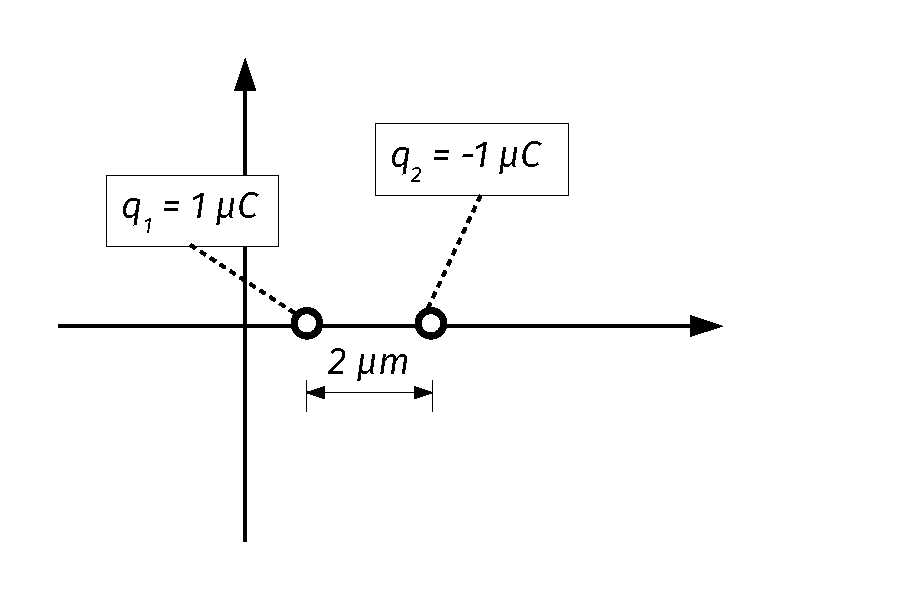
\includegraphics[width=0.5\textwidth]{midtermDiagram1.pdf}
\caption{\label{fig:fig1} Two charges separated by a given distance.}
\end{figure}
\begin{enumerate}
\item What is the magnitude of the force between the charges? \\ \vspace{2cm}
\item In which direction is the force?
\begin{itemize}
\item A: To the right for both charges
\item B: To the left for both charges
\item C: The force on $q_1$ is to the right, the force on $q_2$ is to the left
\item D: The force on $q_2$ is to the right, the force on $q_1$ is to the left
\end{itemize}
\item Suppose the charges are \textit{bound}, meaning that although there is a force acting on them, they do not accelerate.  Add another charge to Fig. \ref{fig:fig1} such that the net Coulomb force on one of the charges is zero.  Give the location and magnitude of the charge. \\ \vspace{2cm}
\end{enumerate}
\item \textbf{Distributions of charges and the electric field.} A positive charge $q_1$ is located in a $x-y$ coordinate system at (0,0).  Recall that the relationship between the Coulomb force and the electric field is $\vec{F}_C = q\vec{E}$ for some test charge $q$.  See Fig. \ref{fig:fig2}.
\begin{figure}[hb]
\centering
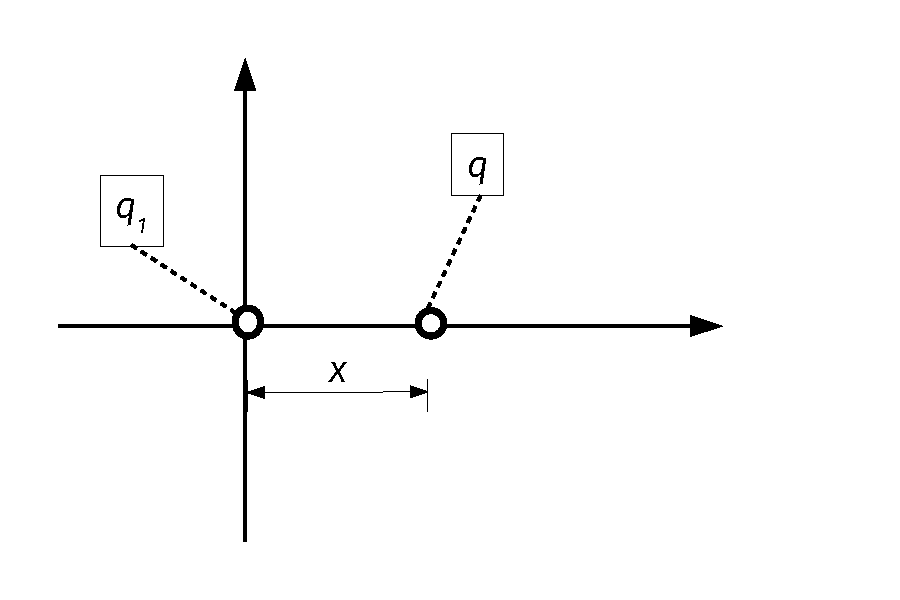
\includegraphics[width=0.5\textwidth]{midtermDiagram2.pdf}
\caption{\label{fig:fig2} Two charges separated by a given distance.}
\end{figure}
\begin{enumerate}
\item Write an expression for the electric field $\vec{E}$ at the location $P = (x,0)$, where $x>0$.  In what direction does the electric field point?  \\ \vspace{1cm}
\item Add another positive charge $q_2$ at the location $(2x,0)$ to Fig. \ref{fig:fig2}.  What is the distance between a test charge located at $x$ and the charge $q_2$? \\ \vspace{1cm}
\item Write a new expression for the electric field at the point $(x,0)$.  What is the value of the electric field if $q_1 = q_2$? \\ \vspace{2cm}
\end{enumerate}
\item \textbf{Drawing electric field lines, 1.} Recall our experience with the PHeT simulation of charges and fields.  (a) Create a charge distribution of negative charges in a straight line, and another distribution of positive charges in a straight line.  Make the two lines of charge parallel. (b) Illustrate the correct electric field between the charge distributions by drawing electric field lines. \\ \vspace{4cm}
\item \textbf{Drawing electric field lines, 2.} Recall our experience with the PHeT simulation of charges and fields.  (a) Create a charge distribution of positive charges, such that if you were to rotate the page by 90 degrees, the electric field would be the same.  (b) Add charges such that the electric field would not change if the page were rotated by 45 degrees instead of 90 degrees.  \\ \vspace{4cm}
\item \textbf{Electric potential and electric field.} Recall that the relationship between a uniform electric field $E$ and the associated change in voltage $V$ is $V = Ed$, where $d$ is a distance.  Two uniformly charged plates with charges $+Q$ and $-Q$ create a uniform electric field $E$ between them.  Let the voltage at the negatively charged plate be 0 V.
\begin{enumerate}
\item 	If the distance between the plates is 1 mm, and the electric field has a value of 10 V/mm, what is the voltage at the positive plate? \\ \vspace{1cm}
\item Draw a graph of the voltage versus the distance between the two plates. \\ \vspace{3cm}
\end{enumerate}
\item \textbf{Capacitors, and capacitance.} Recall that the charge $Q$ stored on a capacitor is $CV$ for a given potential $V$, and that the unit of capacitance is the \textit{Farad}, F.
\begin{enumerate}
\item How much charge is stored on a capacitor with $C = 1\mu$F, if the voltage is $V = 5$ V? \\ \vspace{0.75cm}
\item Two capacitors each have a $1\mu$F capacitance, and are connected \textit{in series}.  What is the total capacitance?  \\ \vspace{0.75cm}
\end{enumerate}
\item \textbf{Definition of current, resistance, and Ohm's Law} Recall that \textit{current} is the change in charge per unit time, $I = \Delta Q/\Delta t$, and that the unit of current is the \textit{amp}, A, which is 1 C/s.  Also recall that Ohm's Law is $V=IR$, where $V$ is the voltage, $I$ is the current, and $R$ is the total effective resistance.
\begin{enumerate}
\item How much current flows through a circuit that lights a lightbulb, if the voltage is 12 V, and the lightbulb has a resistance of $10$ Ohms?
\begin{itemize}
\item A: 1.2 V
\item B: 1.2 amps
\item C: 12 amps
\item D: 12 V
\end{itemize}
\item Recall that the relationship between the power $P$ consumed by a resistor drawing a current $I$ while being given a voltage $V$ is $P=IV$.  How many watts is the light bulb consuming?
\begin{itemize}
\item A: 10 watts
\item B: 14 watts
\item C: 20 watts
\item D: 100 watts
\end{itemize}
\vspace{1cm}
\item Draw a graph of voltage versus current for the lightbulb in part (a), assuming the voltage can vary.  Make sure to label the axes of the graph. \\ \vspace{3cm}
\item Suppose the second light bulb is instead connected \textit{in parallel} with the first light bulb.  What is the new current flowing from the battery? What is the new power consumption? \\ \vspace{1.5cm}
\end{enumerate}
\item \textbf{Nerve signals.} Recall the model of nerve signals in the human body as time-dependent chemical capacitors.
\begin{enumerate}
\item As accurately as possible, draw below the \textbf{action potential} of a nerve signal in an axon in the human body.  Label the axes with appropriate units. \\ \vspace{4cm}
\item Write a one-sentence explanation for each of the four stages of the action potential. \\ \vspace{2cm}
\item What is the reason that some nerves have very short \textit{nodes} but longer myelinated sections?  What happens to the amplitude of a nerve signal as it propagates through a myelinated section?  What happens to the speed in a myelinated section relative to nodes?
\end{enumerate}
\end{enumerate}
\end{document}